% This is samplepaper.tex, a sample chapter demonstrating the
% LLNCS macro package for Springer Computer Science proceedings;
% Version 2.21 of 2022/01/12
%
\documentclass[runningheads]{llncs}
%
\usepackage[T1]{fontenc}
% T1 fonts will be used to generate the final print and online PDFs,
% so please use T1 fonts in your manuscript whenever possible.
% Other font encondings may result in incorrect characters.
%
\usepackage{graphicx}
% \usepackage{subfig}
\usepackage{subcaption}
\usepackage{placeins}
% Used for displaying a sample figure. If possible, figure files should
% be included in EPS format.
%
% If you use the hyperref package, please uncomment the following two lines
% to display URLs in blue roman font according to Springer's eBook style:
%\usepackage{color}
%\renewcommand\UrlFont{\color{blue}\rmfamily}
%\urlstyle{rm}
%
\begin{document}
%
\title{Multi-label music genre recognition based on spectrograms}
%
%\titlerunning{Abbreviated paper title}
% If the paper title is too long for the running head, you can set
% an abbreviated paper title here
%
\author{Bartosz Karpiński \inst{1}}
%
\authorrunning{B. Karpiński}
% First names are abbreviated in the running head.
% If there are more than two authors, 'et al.' is used.
%
\institute{Wrocław University of Technology, Wrocław, Poland
\email{bartosz.karpinski@protonmail.com}}
%
\maketitle              % typeset the header of the contribution
%
% In the current day and age, music surrounds us everywhere and accurate genre classification is important to both the recipients as well as music labels and stores. However, due to many factors, nowadays the genres of songs and albums are not clearly defined, often being mixed on a single record, which would require an approach different from the standard multi-class on, which many of the currently available datasets lack. Additionally, they often suffer from the lack of proper annotations, insufficient size, and inadequate representation of the music landscape. That is why in this work an extensive comparison of various preprocessing methods and ways of handling imbalanced data is performed for a multi-label classification. For the experiments different types of spectrograms extracted from audio files were used, and the dataset was personally acquired and labeled based on the biggest on-line music database, resulting in more than 18000, multi-label and representative of current trends data.  

\begin{abstract}
In the current day and age, music surrounds us everywhere and accurate genre classification is important to both the recipients as well as music labels and stores. However, due to many factors, nowadays the genres of songs and albums are not clearly defined, often being mixed on a single record, which would require an approach different from the standard multi-class on, which many of the currently available datasets lack. In addition, they often suffer from the lack of proper annotations, insufficient size, and inadequate representation of the music landscape. That is why in this work an extensive comparison of various preprocessing methods and ways of handling imbalanced data is performed for a multi-label classification. For the experiments different types of spectrograms extracted from audio files were used, and the dataset was personally acquired and labeled based on the biggest on-line music database, resulting in more than 18000, multi-label and representative of current trends data.


\keywords{Multi-Label Classification \and Acoustic Data Classification \and Imbalanced Data Classification}
\end{abstract}



\section{Introduction}
\subsection{Multi-label nature of music}
Music has accompanied humans throughout history, starting with primitive sounds to beautifully complex, classical compositions. However, in modern day and age, the number of new releases each year is constantly increasing. Looking, for example, at one of the biggest online music databases, namely Discogs, we can see how in the 1950s it was around 400 thousands and in the 2010s: more than 4 million. With increased numbers also came increased diversity in the sense of genres. New technologies, especially computer software, drastically changed what can be achieved and created, leading to more and more experimentation, and as a result: subgenres. Oftentimes they start as a slight variation, in time gaining more noticeable, distinct features that differentiate it from its predecessors. Sometimes, it is a result of cross-genre mixing, for example, a rock song with incorporated jazz instrumentation. In such instances, if we were to try to match that release to one more general genre, a case can be made for both. Such cases are also not obscure: A great example of this in recent years was Old Town Road by Lil Nas X and Billy Ray Cyrus, which features a rare combination of Hip-Hop and Country music. Some others, while not as mainstream-popular, bring forth innovation and create whole trends through unorthodox genre mixing. One such example is a Sacramento-based group Death Grips, who have shaped the entire 2010’s in the hip-hop underground, through their mix of Hip-Hop, Industrial, Punk, and Experimental. Their influence has even transcended that underground, as it is unquestionable that their works have been an influence for Kanye West’s 2013 album, Yeezus, which has proven to be a commercial and mainstream success. That is why, in the current landscape of music, limiting the belongingness to only one genre is a far too great oversimplification and thus is counterproductive. However, that leads to a completely new issue: data. 

\subsection{Problems with music datasets}
For years in the field of Music Information Retrieval (MIR), the datasets used for various tasks come with different sets of problems. Some have a really small number of samples and a multitude of other issues\cite{gtzan_analysis}(GTZAN\cite{gtzan}), some lack raw music files (Million Songs Dataset\cite{million}), and others lack proper annotations (MagnaTagATune Dataset). Two other, major issues present in most, if not all, datasets is that they are inadequate for multi-label classification due to their tagging policy, and the tags present are of questionable quality and source (like Amazon shop). Another important aspect is the proper representation: in order to provide most value to the real-life scenarios, the data should reflect the existing landscape: containing modern music with adequate representation of popular genres. Thus, the basis for these experiments comes from the self-aggregated dataset which addresses each of the aforementioned problems. It contains more than 1400 albums, amounting to over 18000 songs, which span all the way back from the 1950s up to 2024, with the heaviest emphasis put on the currently dominant genres, like hip-hop, electronic, rock, and pop, while also having a representation of more niche genres, like industrial, folk, or ambient. In total, 16 major genres were distinguished, and each song was paired with up to three different ones. However, as with the real distribution, this dataset can be characterized as imbalanced and thus a difficult one. The most popular and numerous being hip-hop, consisting of around 5600 songs, while jazz is only 237. All the annotations have been obtained from one of the biggest online music databases: RateYourMusic. Thanks to its vast user base, which helps with tagging all the data, it is probably one of, if not the best source of detailed information about the releases. As the data collected are in the form of raw music files, consisting of mostly MP3, but also MP4 and FLAC files, any kind of information can be retrieved and any transformations can be applied, as needed. 

\section{Related works}

The task of classifying music genres has been approached in many ways over the years. Tzanetakis and Cook ~\cite{gtzan} was one of the first works to show the music genre classification as a pattern recognition task. The authors proposed three sets of characteristics: timbral texture, rhythmic content, and pitch content. The classification itself was performed using Statistical Pattern Recognition, Gaussian, Gaussian Mixture Models, and k-Nearest Neighbors. Ndou et al. ~\cite{genre_classification_review} conducted a case study of the performance of different classification approaches on the popular GTZAN dataset. Traditional machine learning techniques such as linear logistic regression, support vector machines, random forest, naive Bayes, or k-Nearest Neighbors were compared against each other and against a Convolutional Neural Network. The CNN was also trained in 3 different ways: by using 3 second fragments, 30-second fragments, and spectrograms. The CNN models were unfortunately underwhelming, which, as noted by the authors, may have been influenced by the computational constraints for the research. In Lo and Lin ~\cite{genre_classification_content} showcases the usage of features more known in music theory, such as chords, melody, pitch, or even the frequency of occurrence of specific notes to perform the classification tasks on classical music. 

The use of spectrograms was discussed by Nirmal and Mohan ~\cite{genre_classification_spectrograms}, who compared a self-made newly trained sequential CNN model with a pre-trained model VGG16. In Bahuleyan ~\cite{genre_classification_ml} the usage of CNN models in spectrograms, machine learning models in time domain features, and the combination of both was presented. Here also the VGG16 was used, and for the Machine Learning Algorithms the Linear Regression, Gradient Boosting, Random Forest, and Support Vector Machines. For the ensemble, the combination of VGG16 and Gradient Boosting was used and it achieved the best results of all. Costa et al. ~\cite{cnn_spectrogram} uses and tests representation learning together with Convolutional Networks. In addition to using the spectrograms to perform the classification task, the authors also experimented with the fusion of both learned and handcrafted features to assess the complementarity of those two approaches. 

The use of a CNN and RNN hybrid as Convolutional Recurrent Neural Networks in Choi et al. ~\cite{cnn_recurrent} shows some strong performances. CRNN is a modified CNN model, where the last convolutional layers are replaced with the Recurrent Neural Network model. Silla et al. ~\cite{genre_classification_ml_2} proposes the combination of using the time and space decomposition with ensemble classifiers. K-Nearest Neighbors, Naïve-Bayes, Decision Trees and Support Vector Machines were used on the novel Latin dataset. Schindler and Knees ~\cite{schindler2019multi} tackle the multi-label problem of tagging music by features such as genre, style, mood or theme. Their Deep Neural Models were based on the triplet-network architecture.
 One of the earlier works on the multi-label music genre classification is Lukashevich et al. ~\cite{genre_multi_domain}, which describes different approaches of multi-labeling: for the whole song, by dividing it into separate segments and by dividing into segments while simultaneously dividing into domains, such as Timbre, Rhythm, Melody, and Harmony. A fairly similar approach to detect genre borders was proposed in Nakamura et al. ~\cite{genre_multi_border}, which further adds the possibility of applying a single label classification on each detected segment in order to achieve a multi-label classification for the entire song. 

In Oramas et al. ~\cite{genre_multi_source}, the authors present a comparison of different feature extraction methodologies from audio, text reviews, and image covers, as well as their combinations, showing ways to improve accuracy by implementing approaches that may not sound so obvious at first. Here, the CNN is used on the spectrograms for audio, a Vector Space Model for the text, and a modified version of the ResNet model for the covers. The results show the potential of the multimodal approach. Sanden and Zhang ~\cite{sanden2011enhancing} discuss different ensemble techniques for the specific task of the multi-label classification of music genres. Although using only a simpler machine learning approach, the whole research is very robust, covering multiple datasets and ensemble techniques.

\section{Experimental evaluation}
This section describes the evaluation process designed to answer the following questions:
\begin{itemize}
    \item How different methods of imbalance handling impact the multi-label classification?
    \item How do different methods of preprocessing the audio data impact the multi-label classification?
\end{itemize}
\subsection{Set-up}
\paragraph{Dataset} The basis for the experiments was a self-assembled dataset of songs in different formats (MP3, MP4 or FLAC). Each of the 18019 songs has between 1 to 6 genre tags attached, which were taken from largest community-maintained online music database. The table \ref{table:genres} shows the distribution of songs between genres.

\begin{table}[!htbp]
\centering\caption{Number of songs by genre \label{table:genres}}
\begin{tabular}{|l|l|l|l|l|l|l|l|}% table alignment -> l c r - left, center, right
\hline

Hip-Hop	& 5641  & Electronic & 4680 &  Rock	& 4356  & Pop & 2758 \\
\hline
Psychedelia & 1367 & Metal & 1153 & Dance	& 960 & Punk	& 804 \\
\hline
R\&B	& 801 & Industrial \& Noise	& 788 & Experimental & 694 & Ambient & 687 \\
\hline
Folk & 652 & Classical Music	& 608 & Singer-Songwriter & 474 & Jazz & 278 \\
\hline
\end{tabular}
\end{table}

\paragraph{Data preprocessing}
The data in the experiment is analyzed in two forms: spectrograms (Figure \ref{subfig:default}) and mel scale spectrograms (mel spectrograms) (Figure \ref{subfig:mel}). Spectrogram is a visual representation of signal frequencies over time, and mel scale is a perceptual scale adjusted to human hearing ~\cite{mel_spectrogram}. Additionally, a spectrogram obtained from a reduced audio file (Figure  \ref{subfig:reduced}), and the same spectrograms scaled to fill more space of the same reduced file (Figure  \ref{subfig:reduced_scaled}) were used.

\begin{figure*}[t!]
        \subfloat[Default]{%
            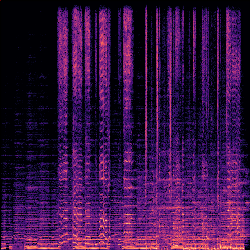
\includegraphics[width=.48\linewidth]{img/default_normal.png}%
            \label{subfig:default}%
        }\hfill
        \subfloat[Mel]{%
            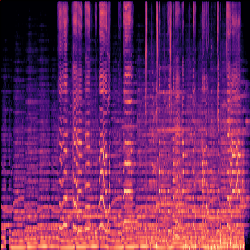
\includegraphics[width=.48\linewidth]{img/default_mel.png}%
            \label{subfig:mel}%
        }\\
        \subfloat[Reduced]{%
            
\includegraphics[width=.48\linewidth]{img/reduced.png}%
            \label{subfig:reduced}%
        }\hfill
        \subfloat[Reduced and scaled]{%
            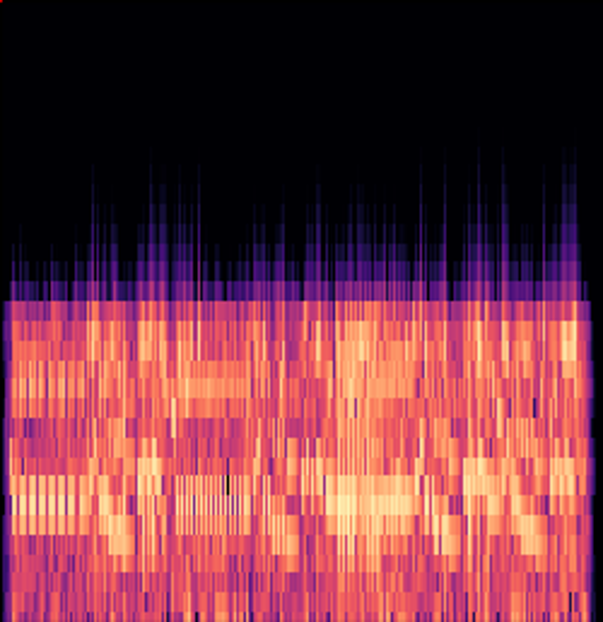
\includegraphics[width=.48\linewidth]{img/scaled.png}%
            \label{subfig:reduced_scaled}%
        }
        \caption{Sample spectrograms of different preprocessing approaches}
        \label{fig:spectrograms}
    \end{figure*}

\paragraph{Model architecture}

The architecture was an ensemble of 16 binary classification models, one per genre, each trained using a \textit{One-vs-All (OVA)} binarization strategy. The model underneath was a custom, self-implemented CNN model.

\subsection{Experimental scenario}

\textbf{Scenario} Comparison of different approaches to handling the imbalanced nature of the data: no imbalance handling, undersampling with shuffling throughout the learning epochs, and shuffling-free stratified undersampling.

\textbf{Goals} Analysis of impact of different techniques to handling the imbalanced dataset problem on the multi-label dataset

\textbf{Scenario} Comparison of different approaches to preprocessing the audio files before extracting spectrograms: default files, a reduced audio file, and reduced file scaled. The reduction was performed by taking only one every 64 frequency values at each point in time, and taking the median of it. The effect is an echo-y audio, resembling the original if one knows what it should sound like, otherwise being rather undistinguishable. The scaling applied in the last approach was to simply scale on the y-axis to simply fill more of the space. 

\textbf{Goals} Analysis of impact of an artificial, lossy transformation of the audio data on the multi-label music dataset

\subsection{Evaluation Protocol}
Due to the size of the data set and the number of models that had to be trained, it was ultimately decided not to perform any cross-validation. On the basis of one run, several metrics were used. For singular-genre models: Accuracy, F1 Score, Balanced Accuracy, Precision, and Recall.

\subsection{Reproducibility}
The code was written using \textit{Python} 3.12.7, with CUDA version 12.4. The libraries used included \textit{TensorFlow} 2.16.1, \textit{Librosa} 0.10.2, \textit{scikit-learn} 1.4.2, \textit{Pandas} 2.2.2 and \textit{Matplotlib} 3.9.0, using a computer with 64GB of RAM, a 16-core CPU, and 8448 CUDA cores GPU with 16GB of VRAM available.

\section{Results}
In the following diagrams, different approaches are described as following: 
\begin{figure}
    \centering
    \begin{minipage}{0.45\textwidth}
        \centering
        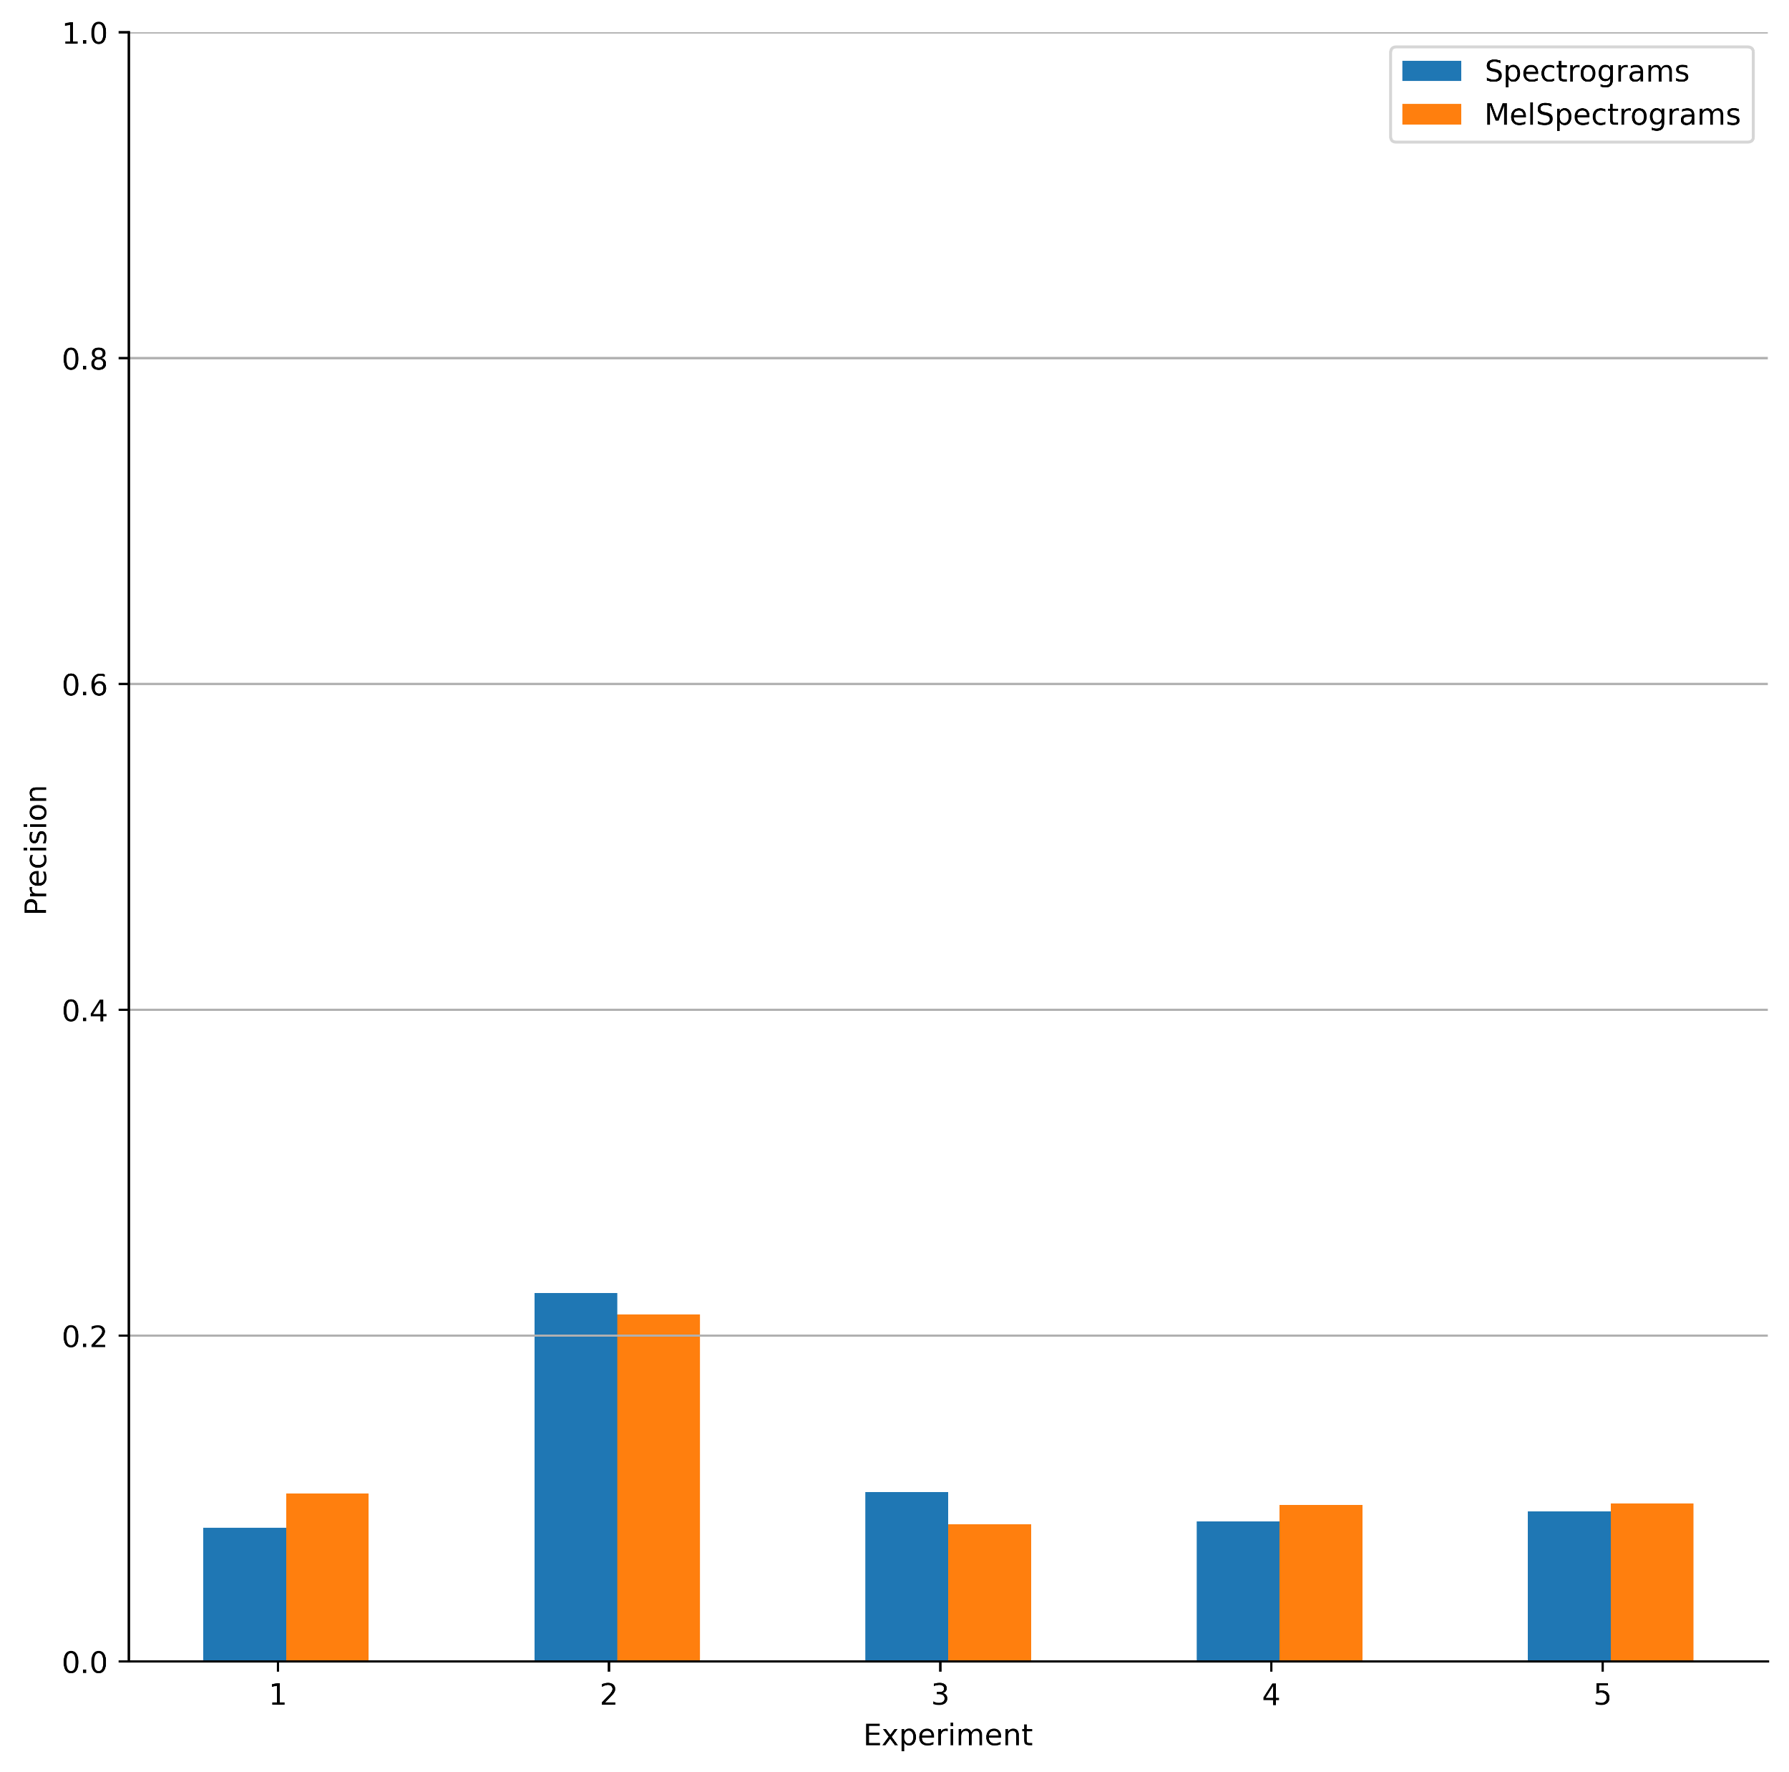
\includegraphics[width=\linewidth]{img/prec.png}
        \caption{Precision scores of different approaches}
        \label{fig:prec}
    \end{minipage}\hfill
    \begin{minipage}{0.45\textwidth}
        \centering
        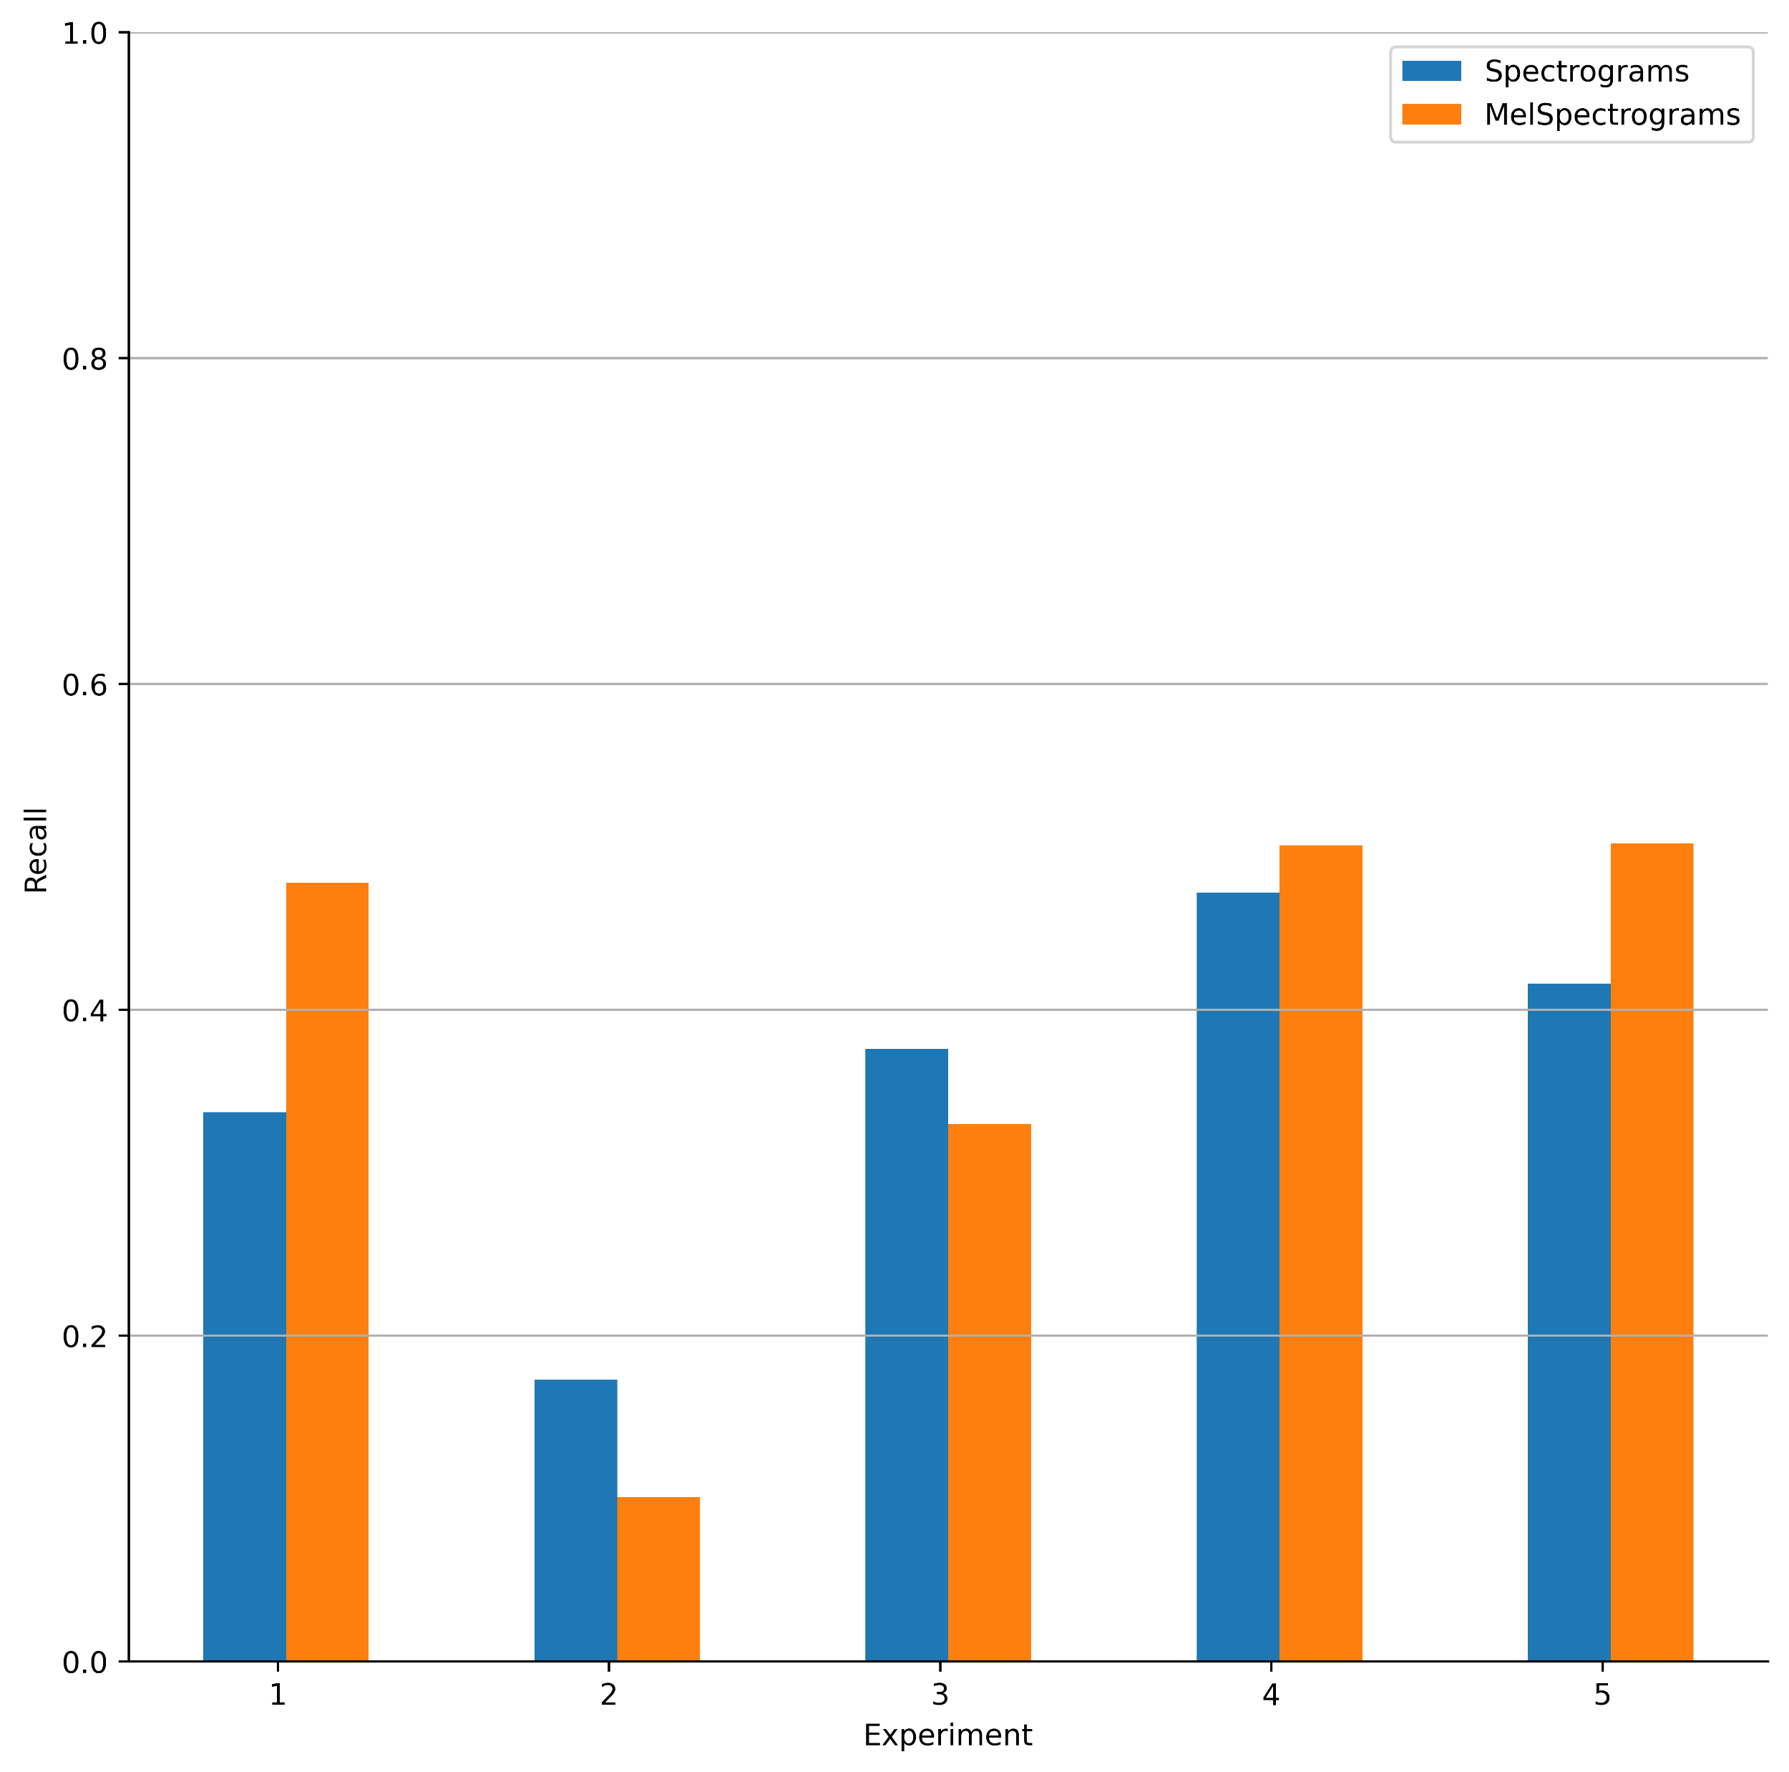
\includegraphics[width=\linewidth]{img/rec.png}
        \caption{Recall scores of different approaches}
        \label{fig:rec}
    \end{minipage}
\end{figure}
\FloatBarrier
shuffling through epochs - experiment 1; no imbalance handling - experiment 2; stratified undersampling - experiment 3;  reduced audio with stratified undersampling - experiment 4; reduced and scaled audio with stratified undersampling - experiment 5. 

On figures \ref{fig:prec} and \ref{fig:rec}, with precision and recall respectively, we can see that all except of the second approach perform similarly, especially with regards to precision. In 3 out of 5 also the mel spectrograms perform slightly better. In the approach with no handling of the imbalance, while precision is noticeably higher than the others, it's a tradeoff with the recall. 

Thus when taking a look at figure \ref{fig:f1} with F1 Score, it all evens out across the board, and also at figure \ref{fig:bac} with the Balanced Accuracy Score, the previous trends of mel spectrograms outperforming the default ones in approaches 1, 4 and 5 continue, as well as the seemingly best scores of approach 2. This is most probably a result of the number of total examples provided to the models at the training time, as due to hands-off approach in the second experiment, all of available training examples were provided, whereas in other approaches only some (rather small) part was used. This proves that another approach, rather than simple stratified undersampling should be used to achieve better results while maintaining the focus on the minority class in each case.   
\begin{figure}
    \centering
    \begin{minipage}{0.45\textwidth}
        \centering
        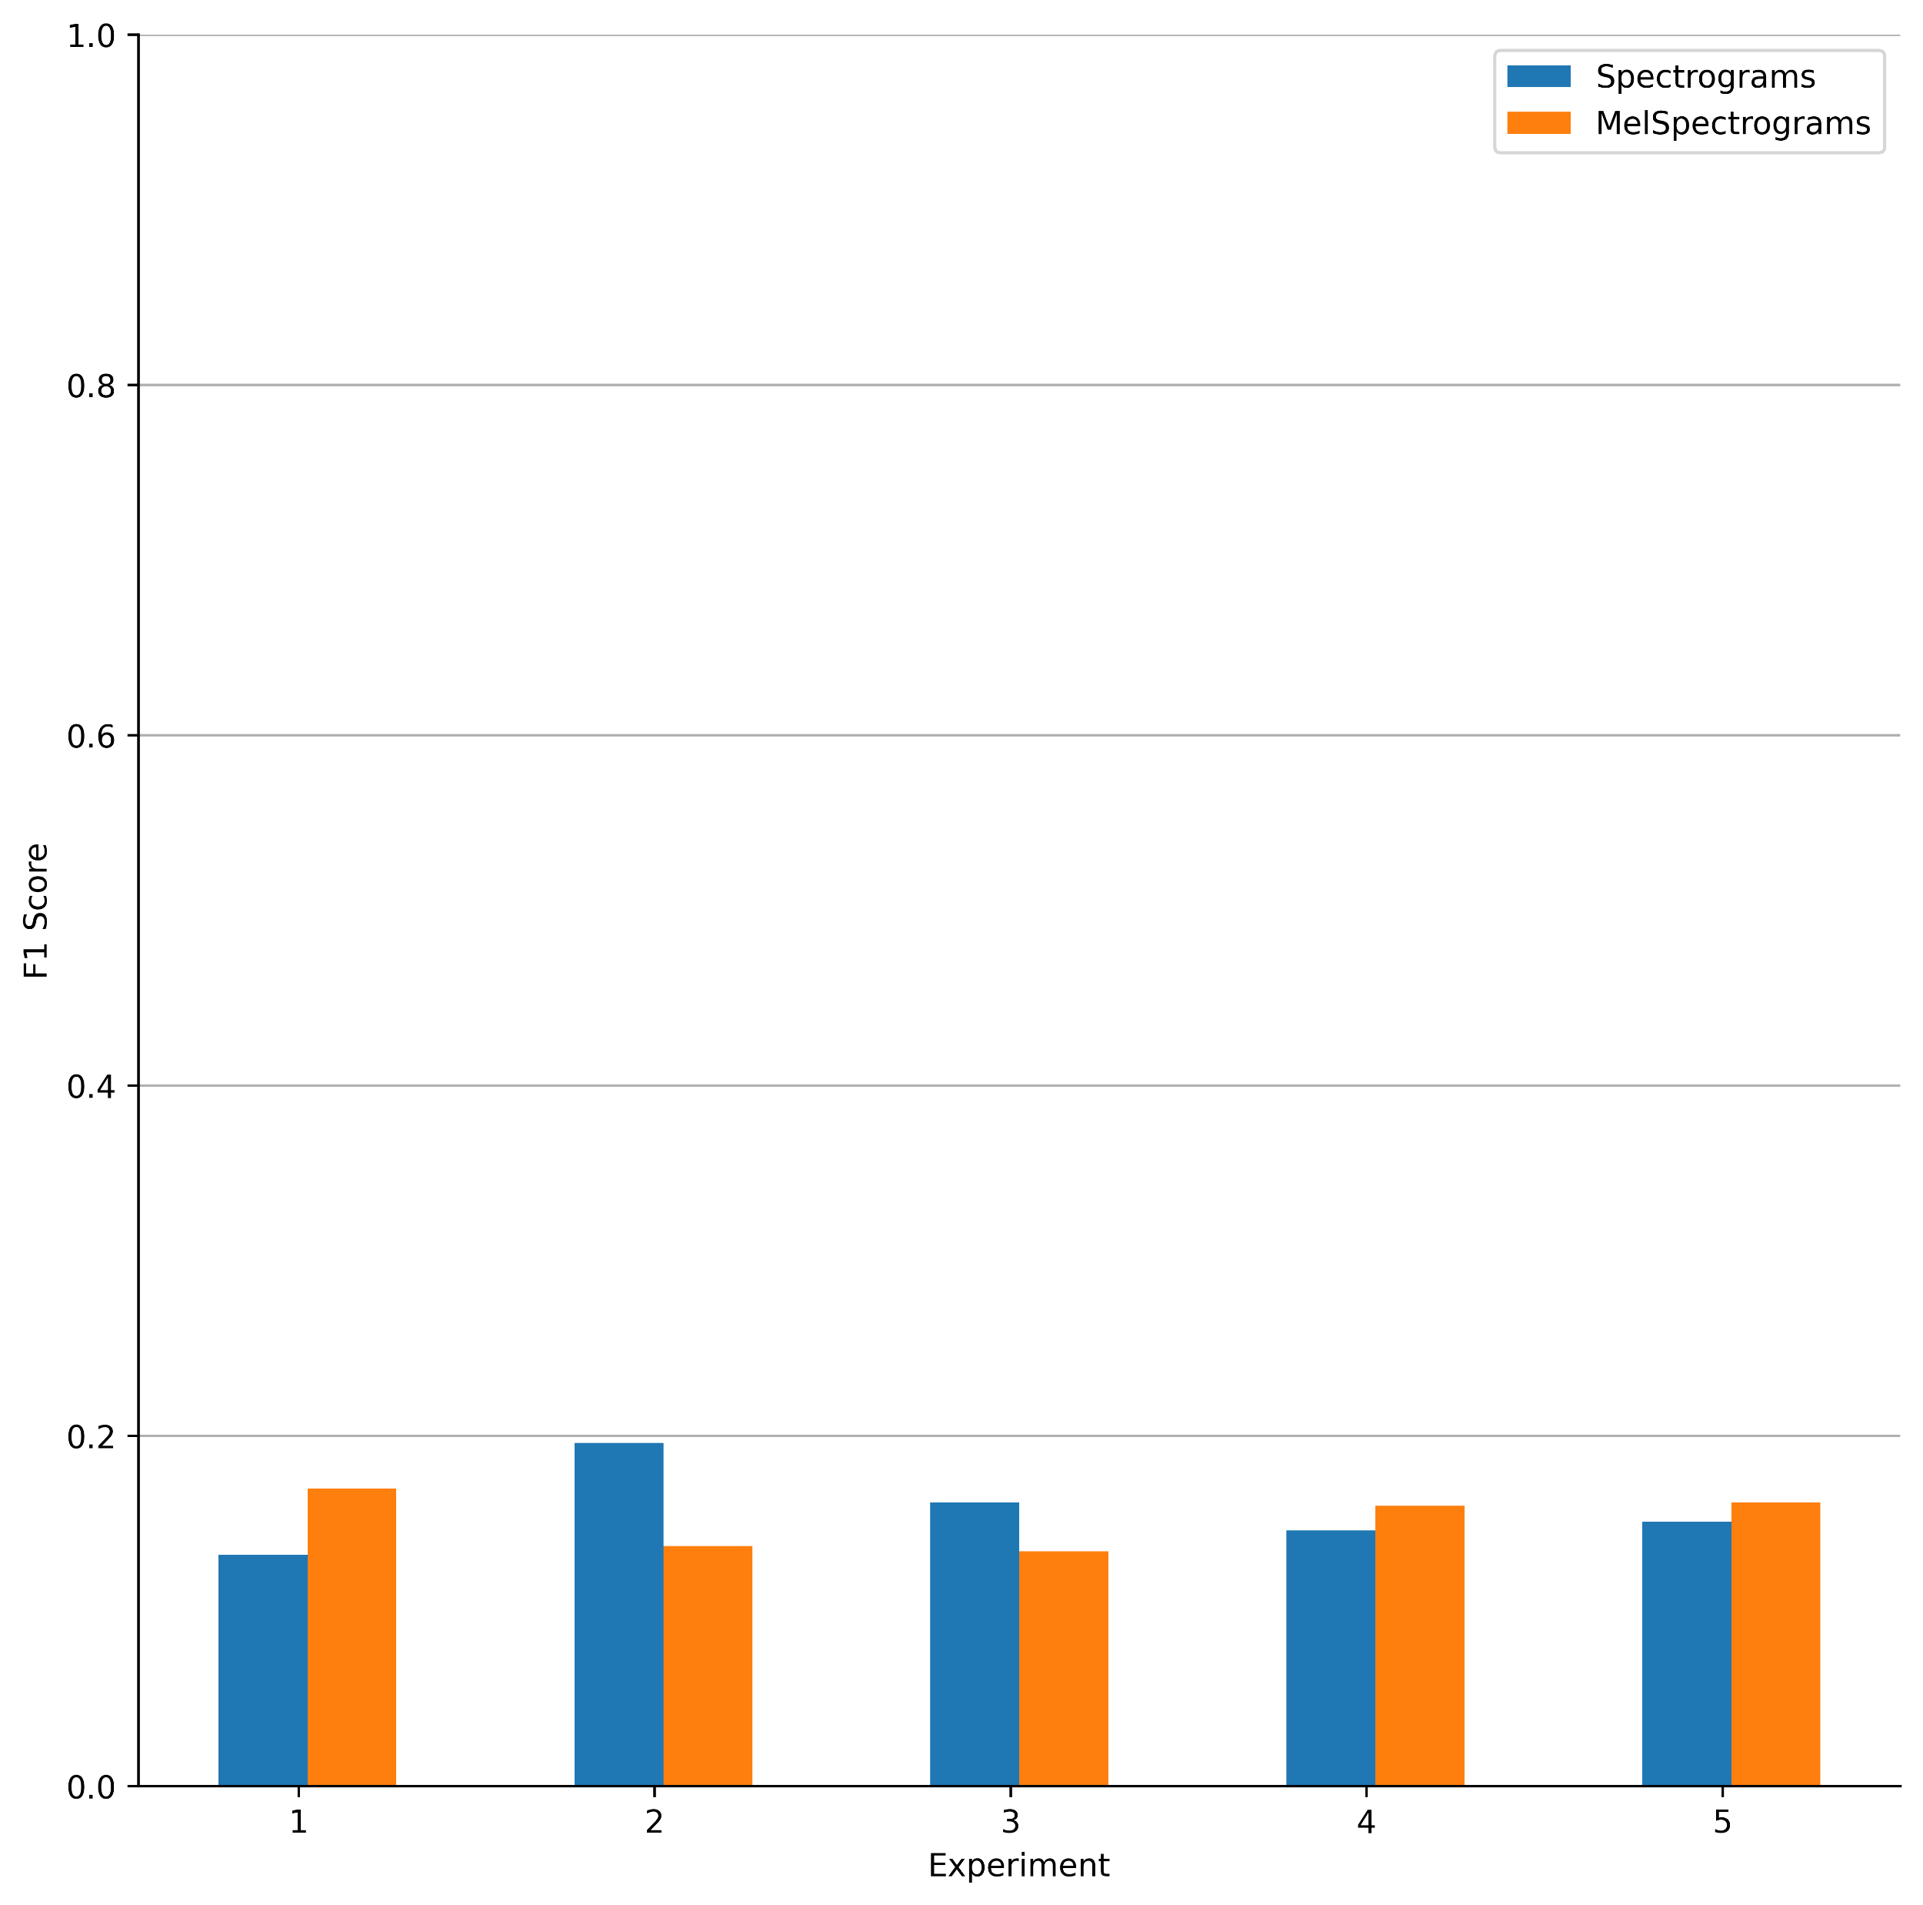
\includegraphics[width=\linewidth]{img/f1.png}
        \caption{F1 scores of different approaches}
        \label{fig:f1}
    \end{minipage}\hfill
    \begin{minipage}{0.45\textwidth}
        \centering
        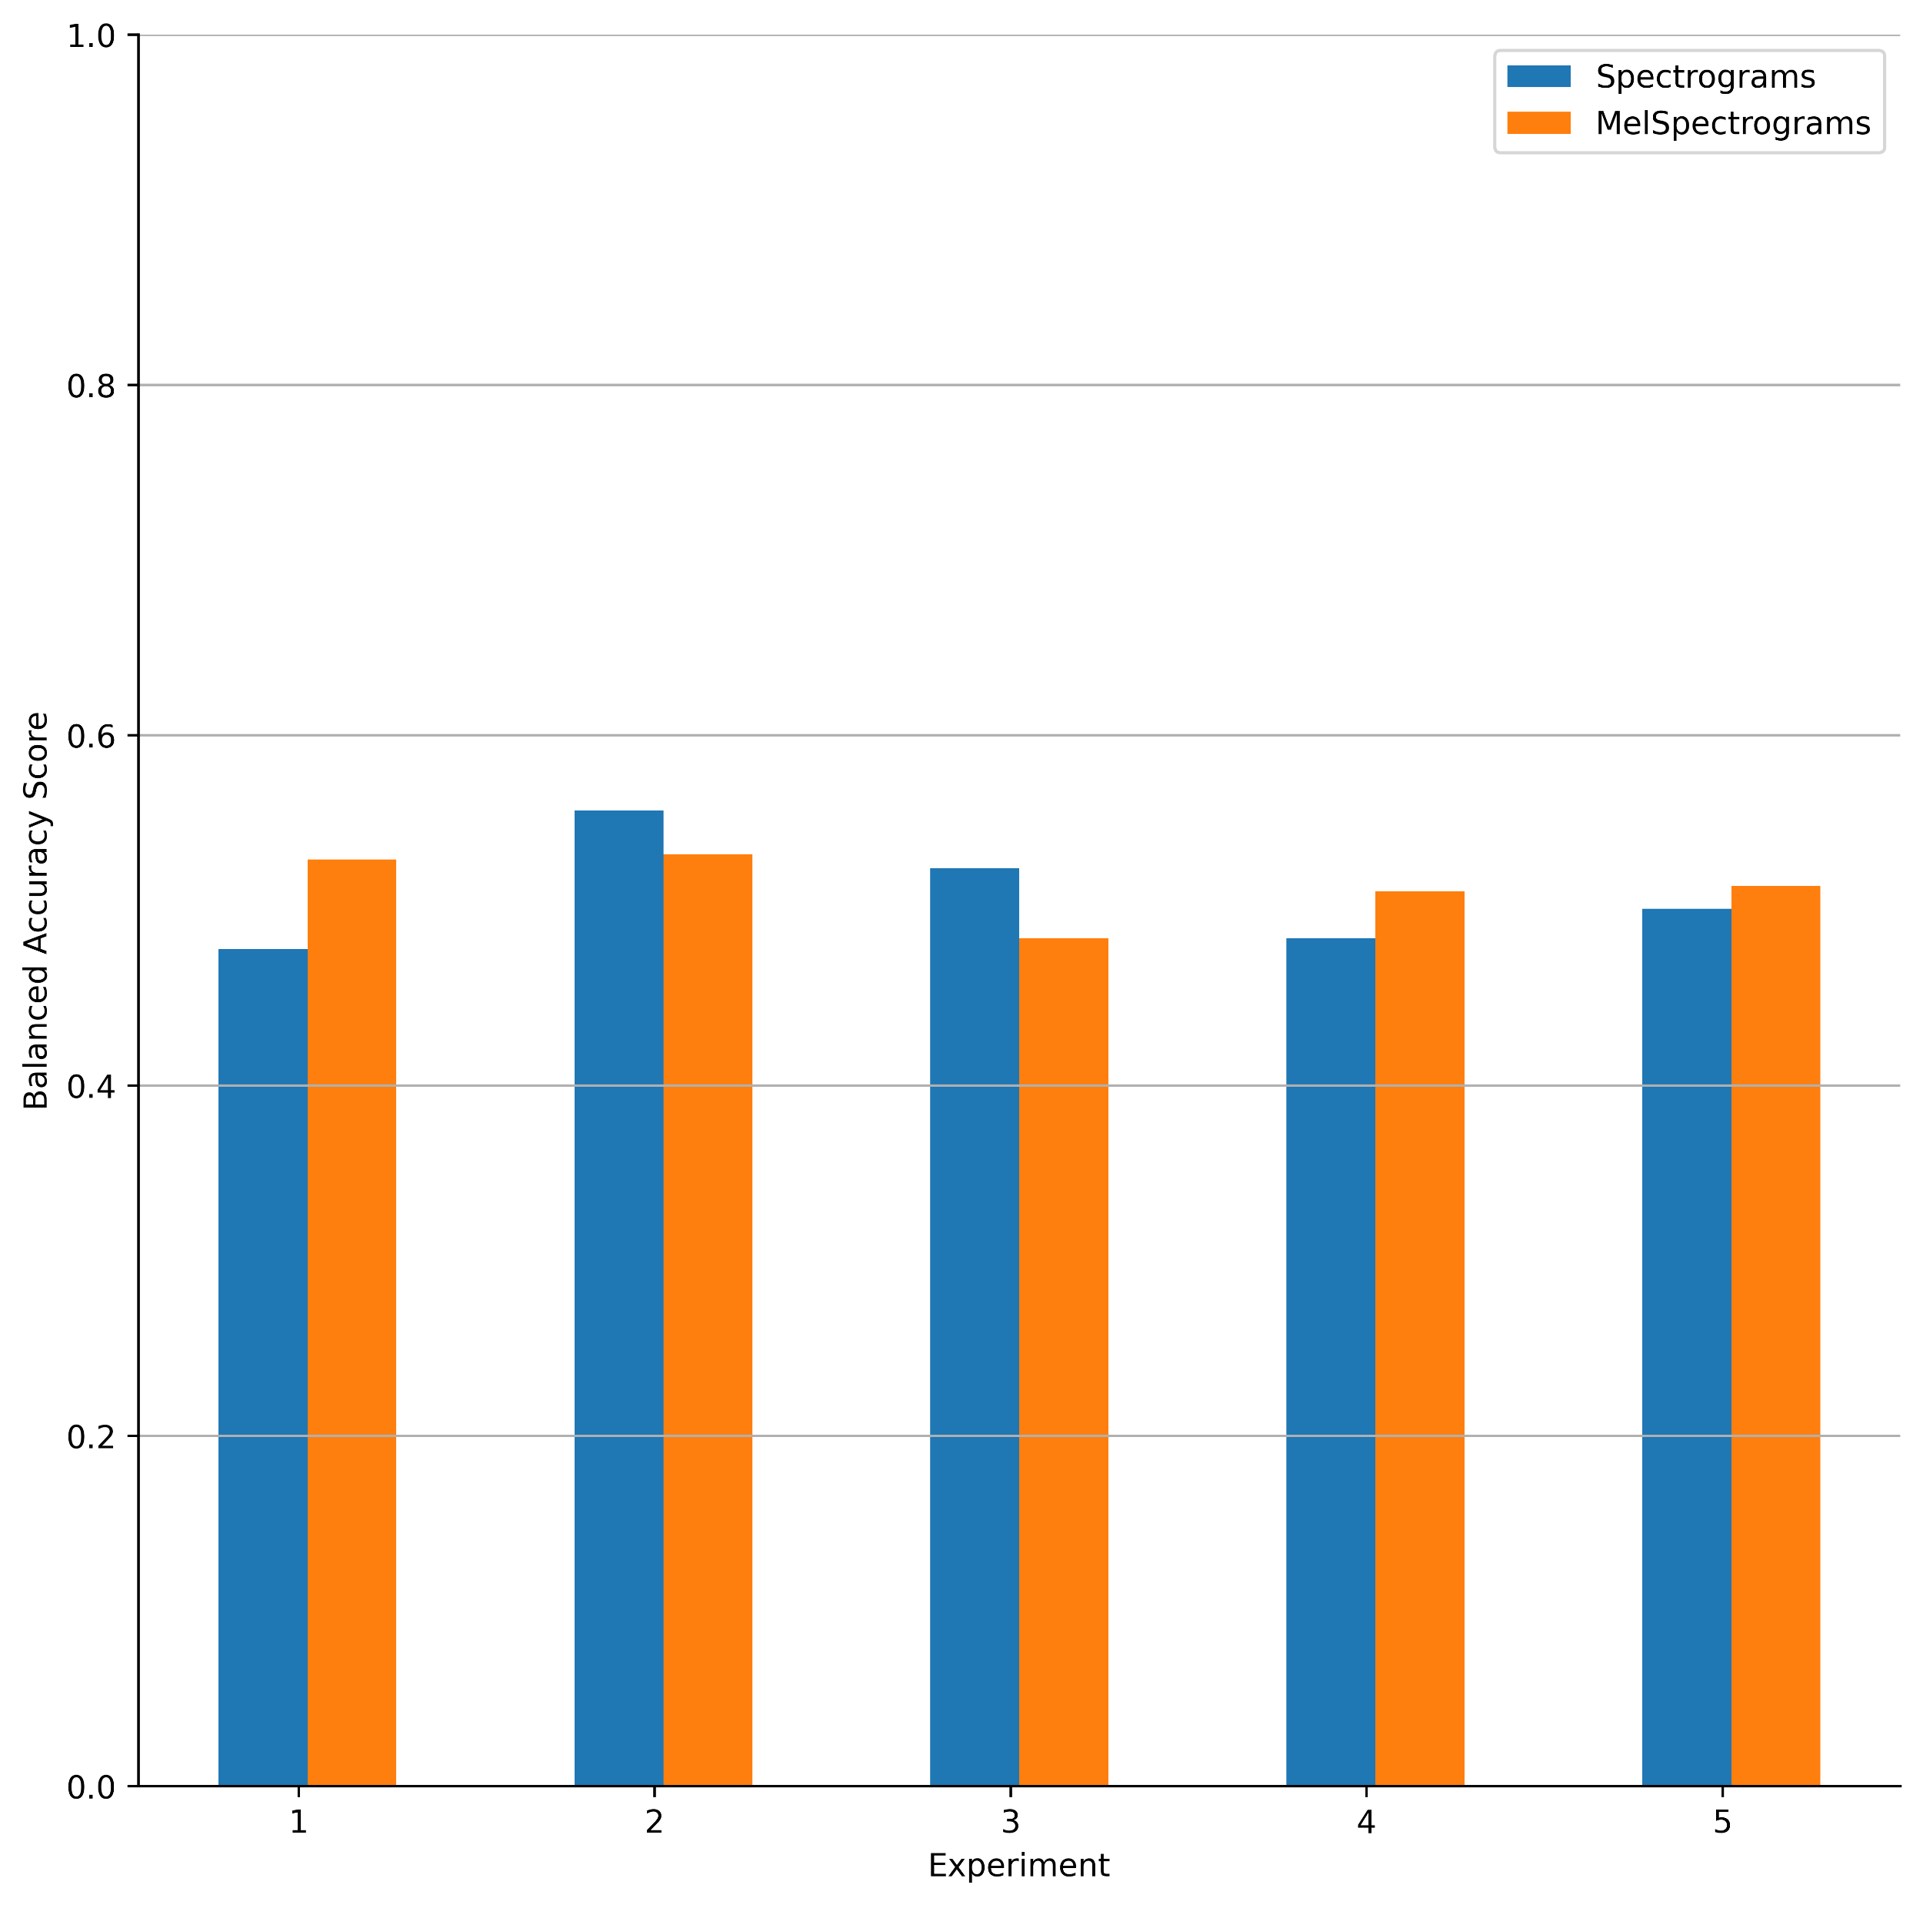
\includegraphics[width=\linewidth]{img/bac.png}
        \caption{Balanced Accuracy scores of different approaches}
        \label{fig:bac}
    \end{minipage}
\end{figure}

However, I believe that most interesting is the comparison between the normal spectrograms and ones achieved from reduced audio files with scaling applied. Looking at the former \ref{fig:ex_3} and the latter \ref{fig:ex_5} figures, the scores achieved across the board are very similar, with the biggest differences being visible in specificity, where the normal files prevail, and in recall, where the situation is turned. Interestingly, the resulting aggregate score such as F1 Score and Balanced Accuracy are very similar, and shows, that even with a lossy transformation of the audio data, the machine learning models are able to extract the features necessary for successful classification no worse than from normal, much larger audio files.

\begin{figure}
    \centering
    \begin{minipage}{0.45\textwidth}
        \centering
        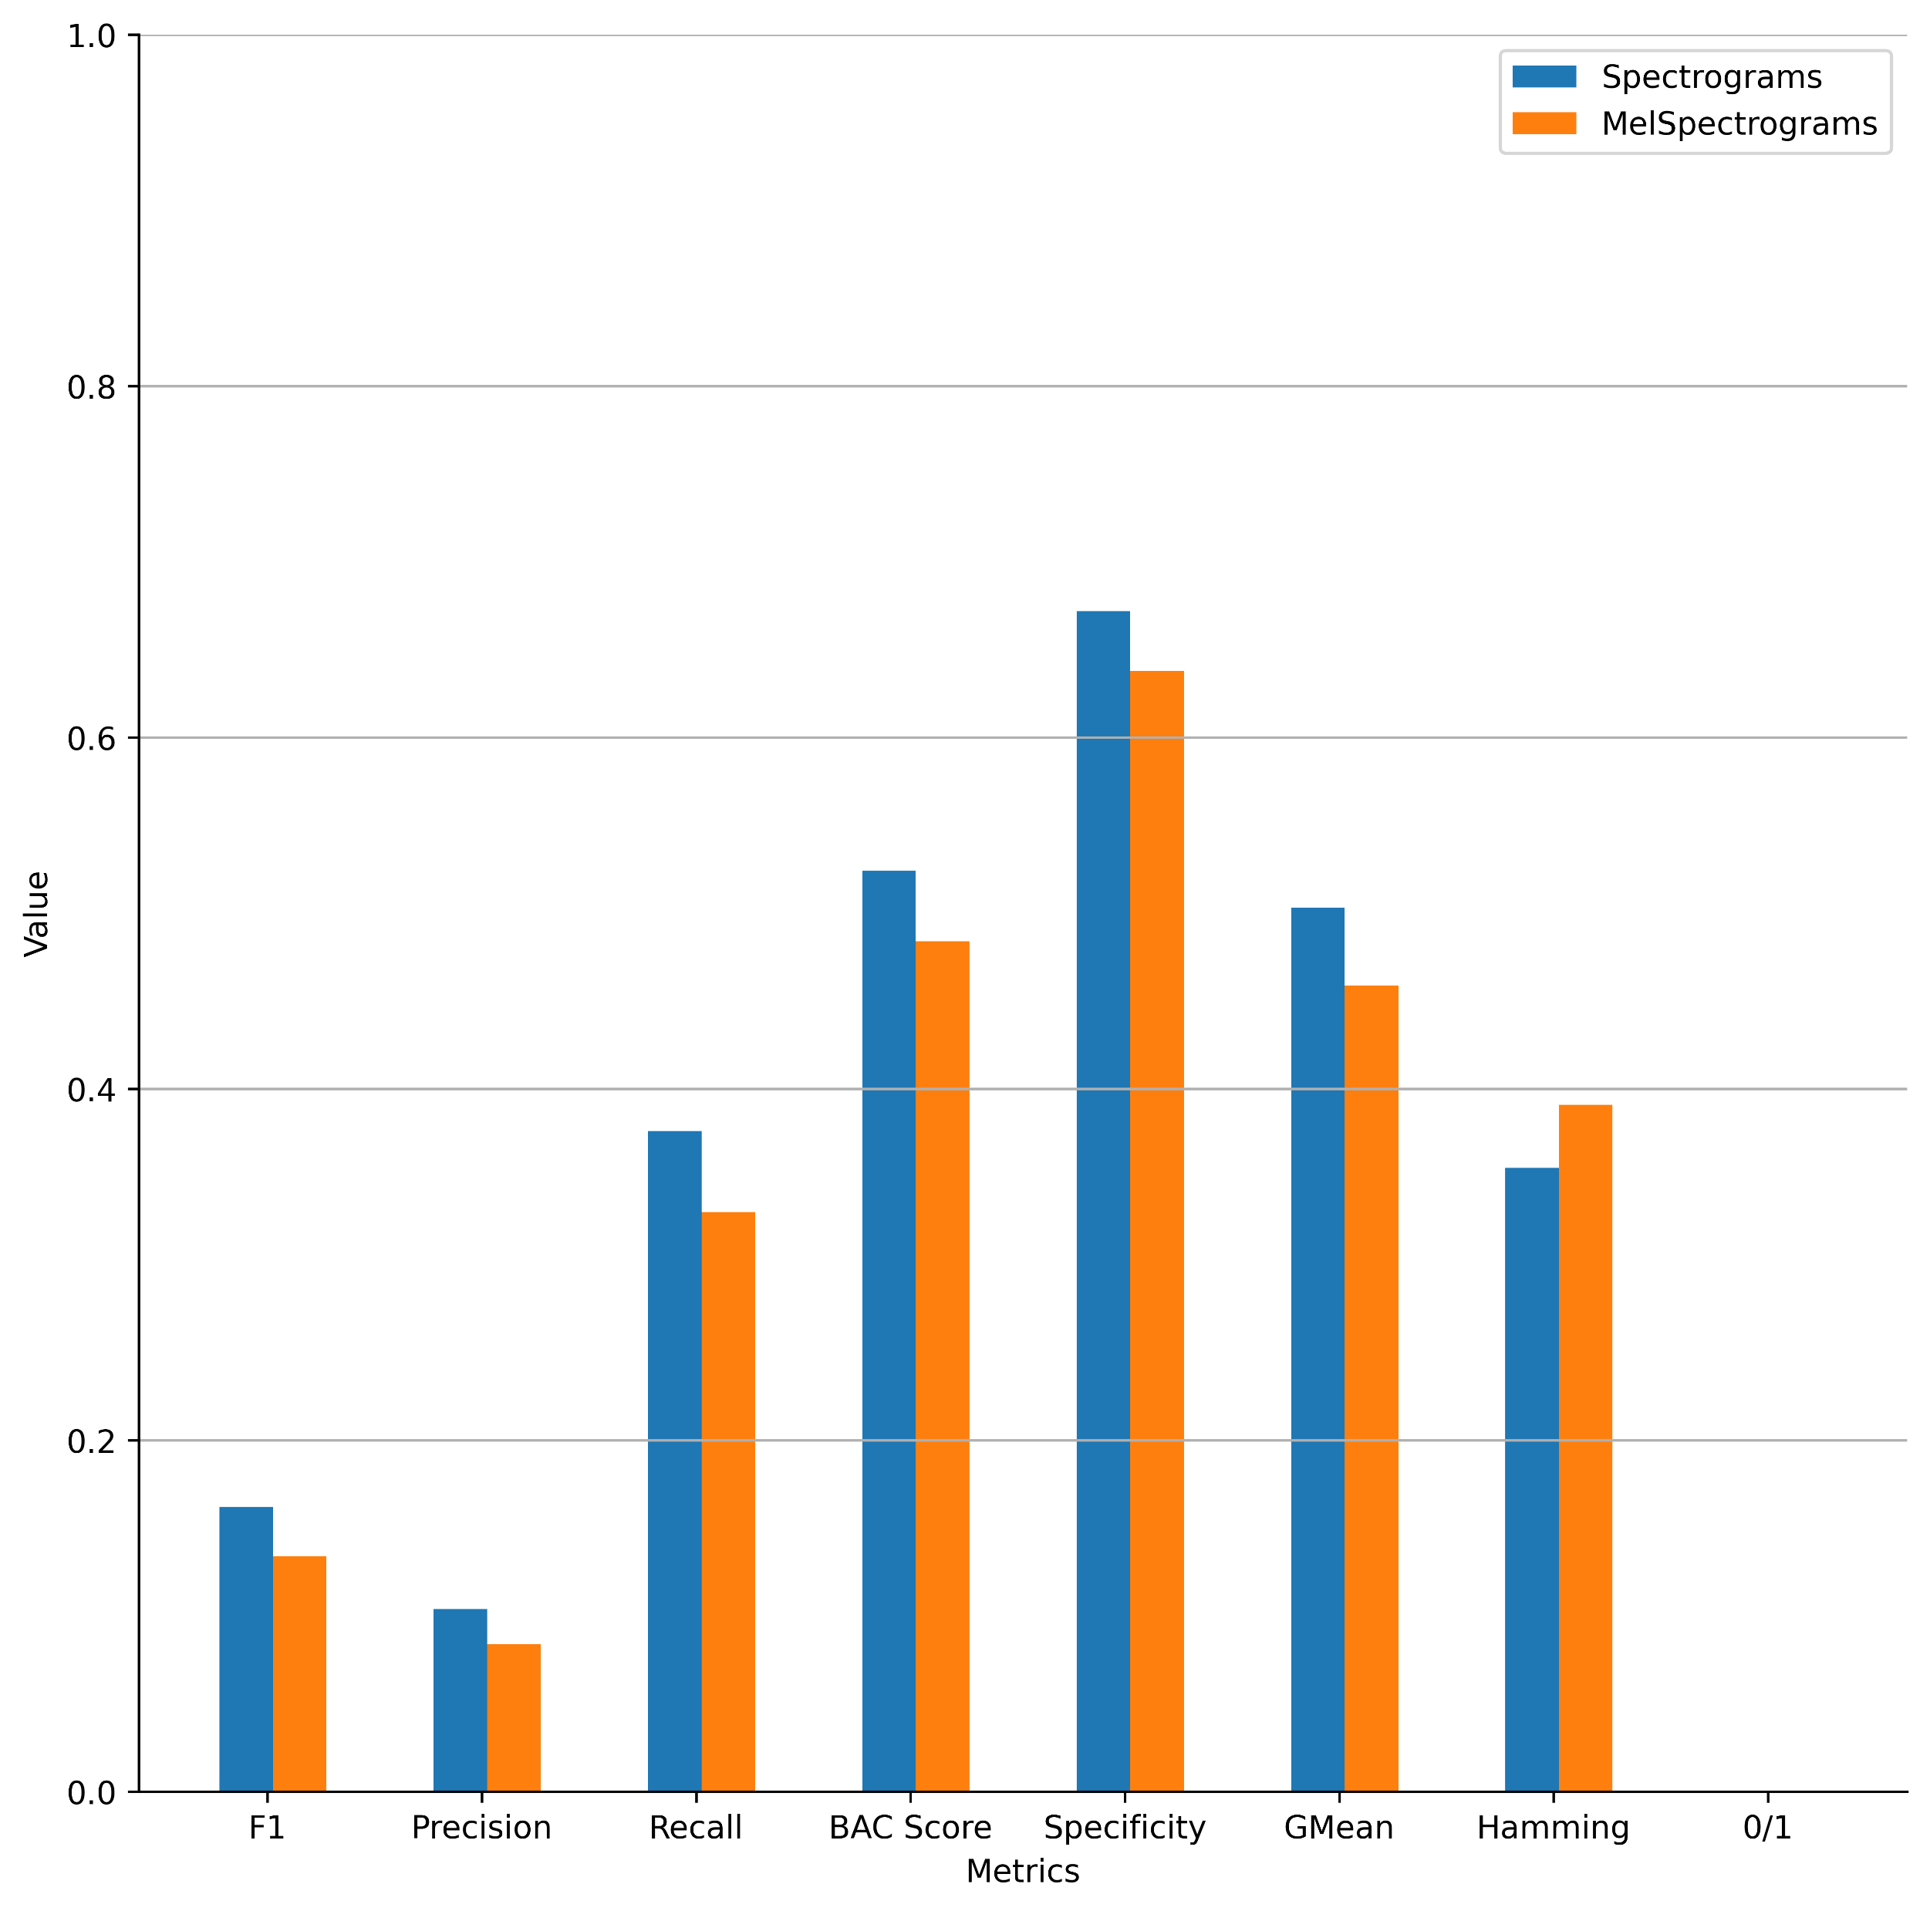
\includegraphics[width=\linewidth]{img/ex3.png}
        \caption{Different scores in the third approach}
        \label{fig:ex_3}
    \end{minipage}\hfill
    \begin{minipage}{0.45\textwidth}
        \centering
        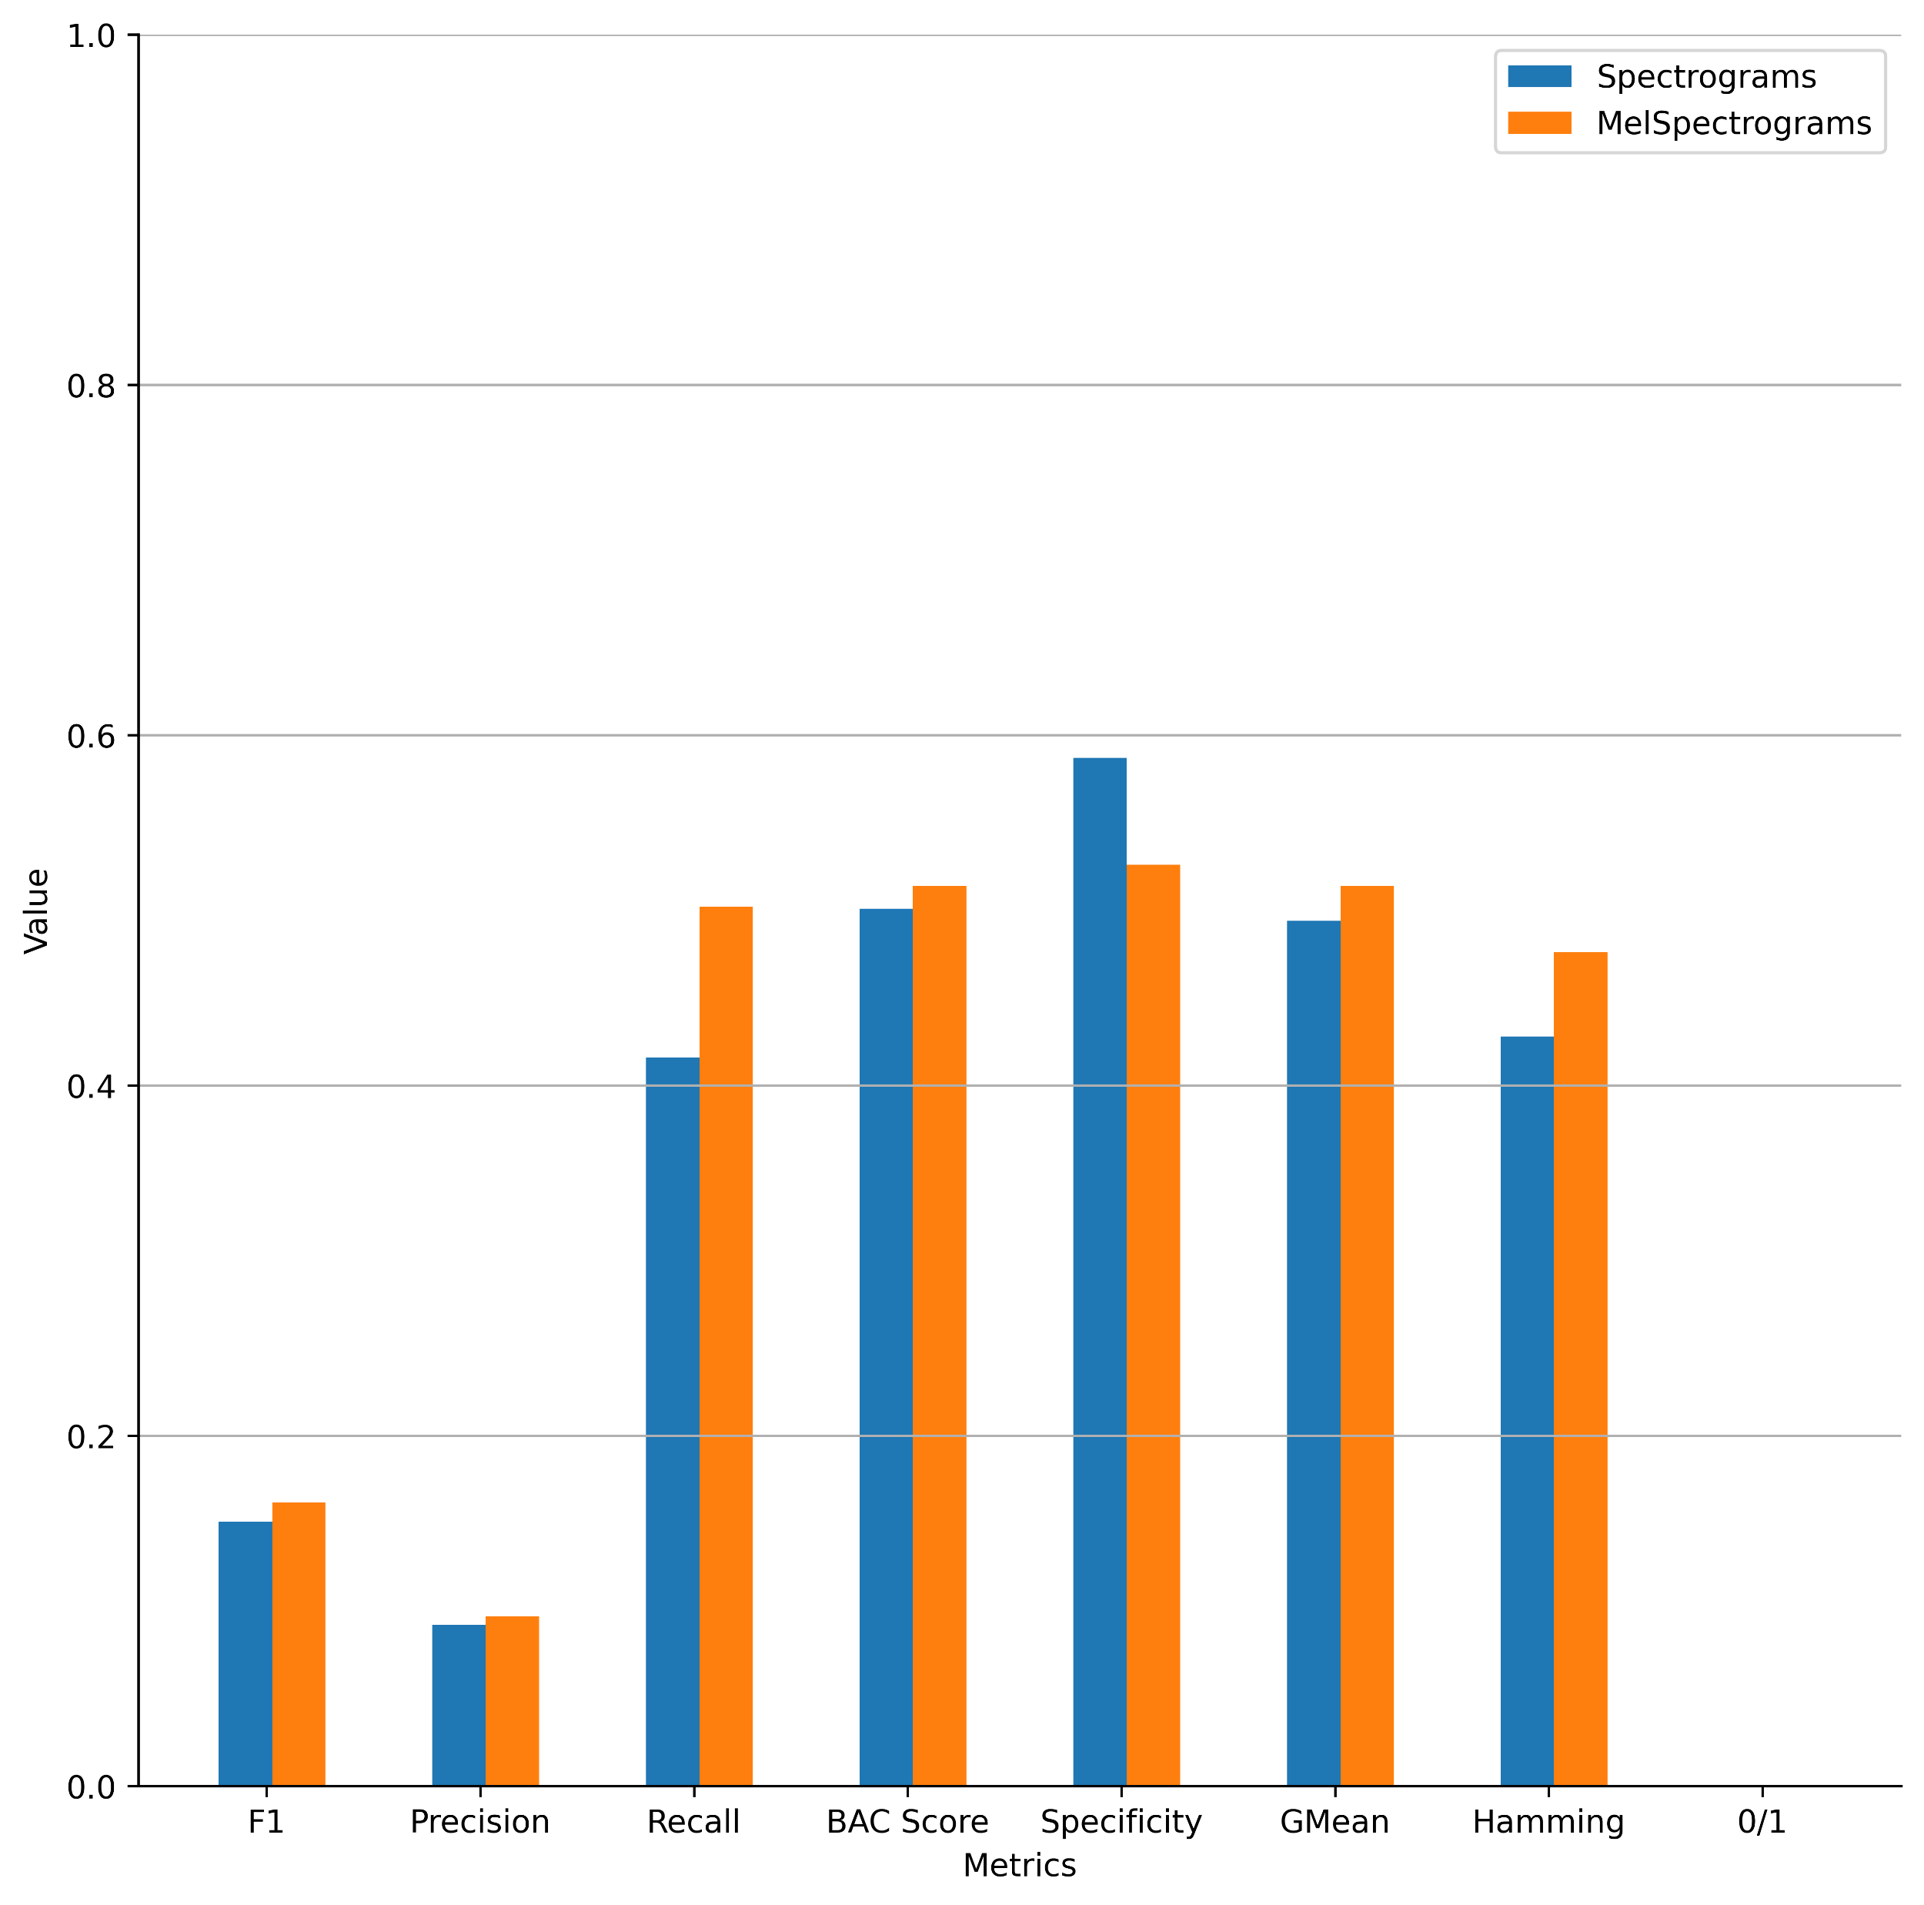
\includegraphics[width=\linewidth]{img/ex5.png}
        \caption{Different scores in the fifth approach}
        \label{fig:ex_5}
    \end{minipage}
\end{figure}

\section{Conclusions and future research}
The general scores achieved by the trained models are rather underwhelming - the aggregate scores such as F1 being in the range between 0.1 and 0.2. This can be most likely attributed to the simplistic nature of the CNN architecture used for the experiments, and thus easily fixable in the future works, by utilizing pretrained and more complex state-of-the-art models such as Resnet or VGG. Despite that fact the conclusions that can be extrapolated from this work are very interesting: the artificial and lossy preprocessing of the audio files can bring competitive results when compared with standard audio files. However, the question of comparison of default and mel spectrograms still stands: more robust models would probably bring more definitive results in that matter. An interesting direction where the future research could be taken would be to perform similar experiment on different state-of-the-art non-CNN solutions, like transformers and state space models, namely Audio Spectrogram Transformer ~\cite{gong2021ast} and Audio Mamba ~\cite{lin2024audio}.

%
% ---- Bibliography ----
%
% BibTeX users should specify bibliography style 'splncs04'.
% References will then be sorted and formatted in the correct style.
%
\bibliographystyle{splncs04}
% \bibliography{mybibliography}

\begin{thebibliography}{8}
\bibitem{mel_spectrogram}
Stevens, S., Volkmann, J., Newman, E.: A scale for the measurement of the psychological magnitude pitch. The journal of the acoustical society of America \textbf{8}(3), 185--190 (1937)
\bibitem{gtzan_analysis}
Sturm, Bob L. "The GTZAN dataset: Its contents, its faults, their effects on evaluation, and its future use." arXiv preprint arXiv:1306.1461 (2013)
\bibitem{gtzan}
Tzanetakis, George, and Perry Cook. "Musical genre classification of audio signals." IEEE Transactions on speech and audio processing 10.5 293-302 (2002)
\bibitem{million}
Bertin-Mahieux, Thierry, et al. "The million song dataset." Ismir. Vol. 2. No. 9. (2011)
\bibitem{genre_classification_review},
Ndou, N., Ajoodha, R., Jadhav, A.: "Music genre classification: A review of deep-learning and traditional machine-learning approaches", IEEE International IOT, Electronics and Mechatronics Conference (IEMTRONICS) 1-6 (2021)

\bibitem{genre_classification_content}
Lo, Y., Lin, Y.: "Content-based music classification" 3rd International Conference on Computer Science and Information Technology, 2 112-116 (2010)

\bibitem{genre_classification_spectrograms}
Nirmal, M., Mohan, S.: "Music genre classification using spectrograms", International conference on power, instrumentation, control and computing (PICC), 1-5 (2020)

\bibitem{genre_classification_ml}
Bahuleyan, H.: "Music genre classification using machine learning techniques", arXiv preprint arXiv:1804.01149 (2018)

\bibitem{cnn_spectrogram},
Costa, Y.,  Oliveira, L. S., Silla Jr, Carlos N. : "An evaluation of convolutional neural networks for music classification using spectrograms" Applied soft computing 52 28-38 (2017)

\bibitem{cnn_recurrent}
Choi, K., Fazekas, G., Sandler, M., Cho, K.: "Convolutional recurrent neural networks for music classification" IEEE International conference on acoustics, speech and signal processing (ICASSP) 2392-2396 (2017)
\bibitem{genre_classification_ml_2},
Silla, C., Koerich, A., Kaestner, C.: "A machine learning approach to automatic music genre classification" Journal of the Brazilian Computer Society 14 7-18 (2008)

\bibitem{genre_multi_domain}
Lukashevich, H., Abe{\ss}er, J., Dittmar, C., Grossmann, H.: "From Multi-Labeling to Multi-Domain-Labeling: A Novel Two-Dimensional Approach to Music Genre Classification": ISMIR 459-464 (2009)

\bibitem{genre_multi_source}
Oramas, S., Nieto, O., Barbieri, F., Serra, X.: "Multi-label music genre classification from audio" Text, and Images Using Deep Features 21 (2017)

\bibitem{genre_multi_border}
Nakamura, H., Huang, H., Kawagoe, K.: "Detecting Musical Genre Borders for Multi-label Genre Classification" IEEE International Symposium on Multimedia 532-533 (2013)


\bibitem{sanden2011enhancing}
Sanden, C., Zhang, J.: "Enhancing multi-label music genre classification through ensemble techniques" Proceedings of the 34th international ACM SIGIR conference on Research and development in Information Retrieval 705-714 (2011)

\bibitem{schindler2019multi}
Schindler, A., Knees, P.: "Multi-task music representation learning from multi-label embeddings" International Conference on Content-Based Multimedia Indexing (CBMI) 1-6 (2019)

\bibitem{lin2024audio}
Lin, J., Hu, H.: "Audio mamba: Pretrained audio state space model for audio tagging" arXiv preprint arXiv:2405.13636 (2024)

\bibitem{gong2021ast}
Gong, Y., Chung, Y., and Glass, J.: "Ast: Audio spectrogram transformer" arXiv preprint arXiv:2104.01778 (2021)

\end{thebibliography}
\end{document}
